\chapter{Sort}


\section{INTRODUCTION}
List of general algorithms:
\begin{enumerate}
\item Selection sort: invariant
\begin{enumerate}
\item Elements to the left of $i$ (including $i$) are fixed and in ascending order (fixed and sorted).
\item No element to the right of $i$ is smaller than any entry to the left of $i$ ($A[i]  \leq\min(A[i+1:n])$.
\end{enumerate}
\item Insertion sort: invariant
\begin{enumerate}
\item Elements to the left of $i$ (including $i$) are in ascending order (sorted).
\item Elements to the right of $i$ have not yet been seen.
\end{enumerate}
\item Shell sort: h-sort using insertion sort.
\end{enumerate}

\section{ALGORITHMS}
\subsection{quick sort}
The key part of quick sort is pivoting:
\begin{python}
def pivot(self, A, i, j):
    """
    Fix the pivot as the 1st element
    In the end, move the pivot to the end of closed set 
    but still inside the closed set, in order to bisect
    pivoting algorithm:
    p | closed set | open set |
    | closed set p | open set |
    """
    p = i
    closed = p
    for ptr in xrange(i, j):
        if A[ptr] < A[p]:
            closed += 1
            A[ptr], A[closed] = A[closed], A[ptr]

    A[closed], A[p] = A[p], A[closed]
    return closed
\end{python}

Notice that this implementation goes $O(N^2)$ for arrays with all duplicates.

\textbf{Problem with duplicated keys}: it is important to stop scan at duplicated
keys (counter-intuitive); otherwise quick sort will goes $O(N^2)$ for the
array with all duplicated items, because the algorithm will put all items
equal to the $A[p]$ on \textbf{a single side}. 

Alternative pivoting implementation with optimization for duplicated keys:
\begin{python}
def pivot_optimized(self, A, lo, hi):
    """
    Fix the pivot as the 1st element
    Scan from left to right and right to left simultaneously
    Avoid the case that the algo goes O(N^2) with duplicated keys
    """
    p = lo
    i = lo
    j = hi
    while True:
        while True:
            i += 1
            if i >= hi or A[i] >= A[lo]:
                break
        while True:
            j -= 1
            if j < lo or A[j] <= A[lo]:
                break

        if i >= j:
            break

        A[i], A[j] = A[j], A[i]

    A[lo], A[j] = A[j], A[lo]
    return j

\end{python}
Applications:
\begin{enumerate}
\item Quick sort.
\item Partial quick sort (selection). 
\end{enumerate}
\section{CONTEXT}
$O(N\lg N)$ is the lower bound of comparison-based sorting; but for other contexts, we may not need $O(N \lg N)$:
\begin{enumerate}
\item Partially-ordered arrays: insertion sort to achieve $O(N)$.
\item Duplicate keys
\item Digital properties of keys: radix sort to achieve $O(N)$.
\end{enumerate}
\section{STABILITY}
Definition: a stable sort preserves the \textbf{relative order of items with equal keys} (scenario: sorted by time then sorted by location). 

Algorithms:
\begin{enumerate}
\item Stable
\begin{enumerate}
\item Merge sort
\item Insertion sort
\end{enumerate} 
\item Unstable
\begin{enumerate}
\item Selection sort
\item Shell sort
\item Quick sort
\end{enumerate}
\end{enumerate}
\textbf{Long-distance swap} operation is the key to find the unstable case during sorting. 
\begin{figure}[hbtp]
\centering
\subfloat{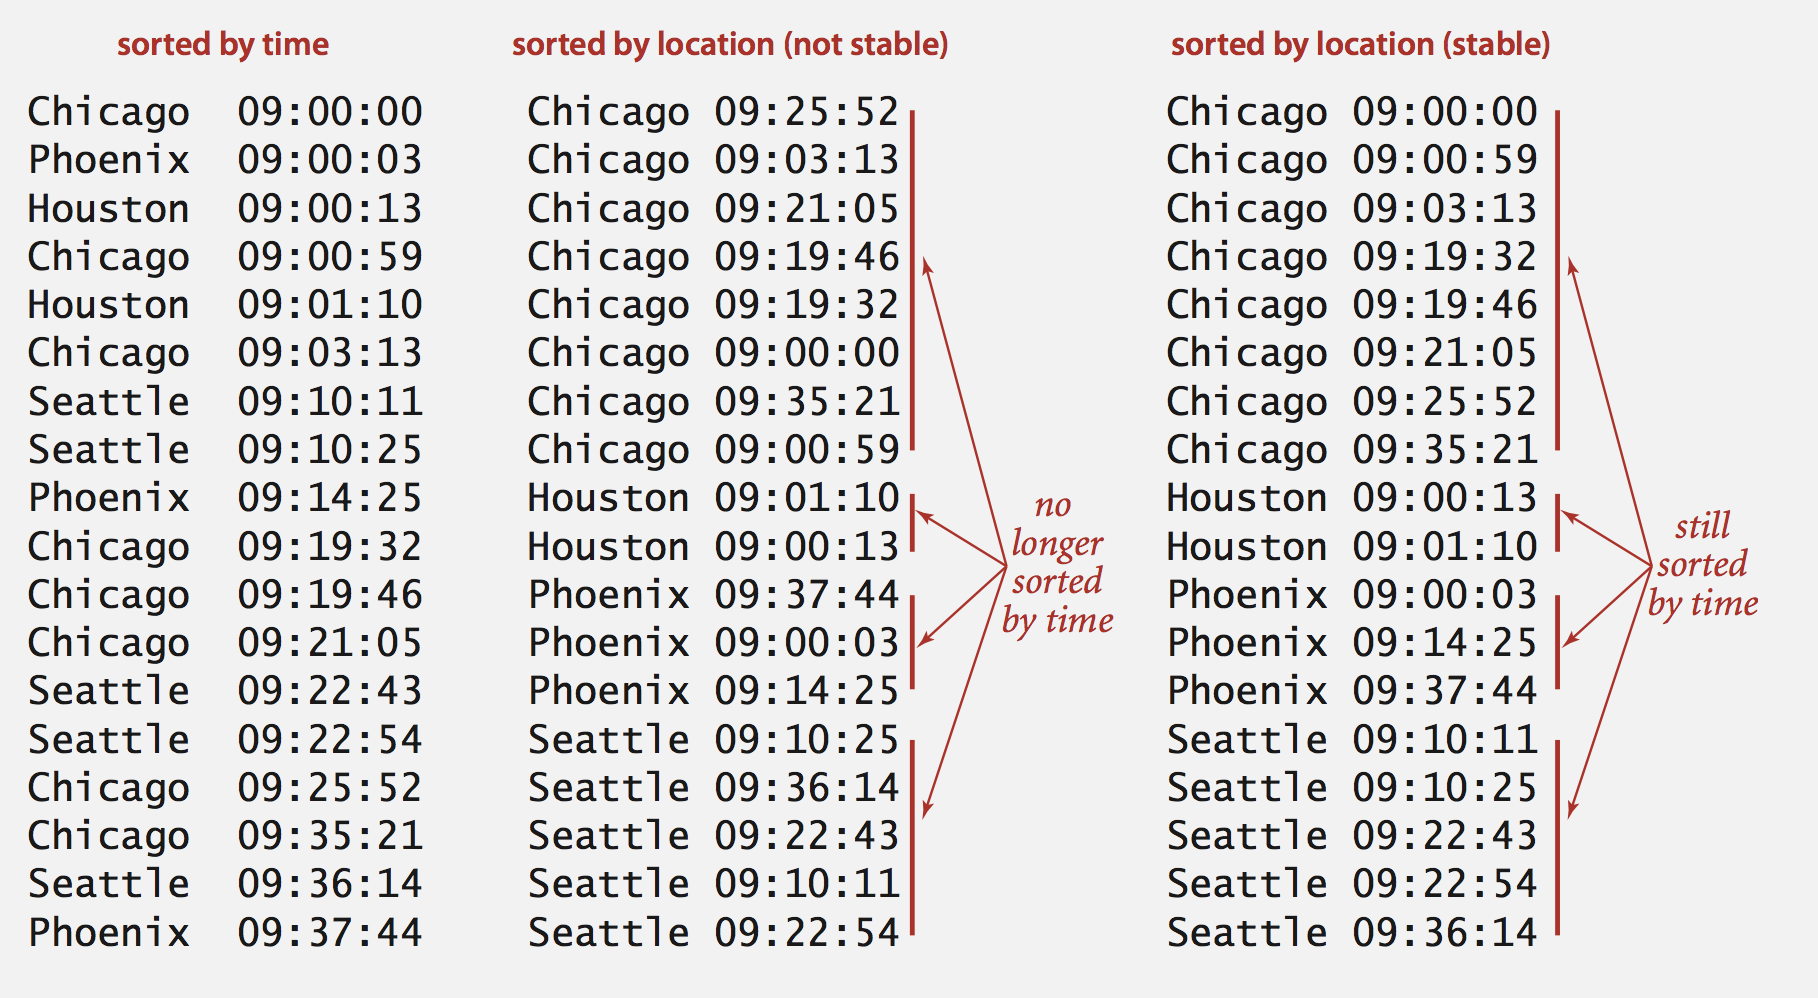
\includegraphics[scale=.60]{stable_sort}}
\caption{Stale sort vs. unstable sort}
\label{fig:trie} 
\end{figure}

